\textbf{Ejemplo 2}
\newline
\newline
Hallar el valor presente de una renta perpetua vencida de 10.000 COP mensuales, suponiendo un interés del 33\% nominal anual mes vencido.\\

%%%%%%%%%%%%%%%%%%% EJERCICIO 1 %%%%%%

%\newpage %USAR SOLO SI EL SOLUCIÓN QUEDA SOLO Y ES NECESARIO BAJARLO A LA SIGUIENTE PAGINA
\textbf{Solución.}
%La tabla ira centrada
\begin{center}
	\renewcommand{\arraystretch}{1.5}% Margenes de las celdas
	%Creación de la cuadricula de 3 columnas \end{flushleft}
	\begin{longtable}[H]{|c|c|c|}
		%Creamos una linea horizontal
		\hline
		%%%%%%%%%% INICIO TITULO
		%Lo que se hace aquí es mezclar las 3 columnas en una sola
		\multicolumn{3}{|c|}{\cellcolor{orange!50}\textbf{1. Asignación del periodo focal}}   \\ \hline
		\multicolumn{3}{|c|}{$pf:0 pmv$} \\ \hline
		\multicolumn{3}{|c|}{\cellcolor{orange!50}\textbf{2. Declaración de variables}} \\  \hline
  
        \multicolumn{1}{|c|}{\cellcolor{orange!50}\textbf{Valores monetarios}}    & \multicolumn{1}{c|}{\cellcolor{orange!50}\textbf{Valores no monetarios}} & \multicolumn{1}{c|}{\cellcolor{orange!50}\textbf{Incógnitas}} \\ \hline
		%%%%%%%%%% FIN TITULO
		%%%%%%%%%% INICIO DE MATEMÁTICAS
		%Cada & hace referencia al paso de la siguiente columna
		$\hspace{1 cm}R=10{.}000\,\,COP\,\,pmv\hspace{1 cm}$ & $\hspace{1 cm}j=33\%namv\equiv i=2.75\%pmv\hspace{1 cm}$ & $VP = ?\,\,COP$ \\ & $n=\infty pmv$ &\\ \hline
		%%%%%%%%%% FIN DE MATEMÁTICAS
		%%%%% FIN DECLARACIÓN DE VARIABLES

        \newpage
        \hline
  
		%%%%% INICIO FLUJO DE CAJA
		\rowcolor{orange!50}
		\multicolumn{3}{|c|}{\cellcolor{orange!50}\textbf{3. Diagrama de flujo de caja}} \\ \hline
		%Mezclamos 3 columnas y pondremos el dibujo
		%%%%%%%%%%%%% INSERCIÓN DE LA IMAGEN
		%Deberán descargar las imágenes respectivas del drive y pegarlas en la carpeta
		%n_capitulo/img/ejemplos/1/capitulo1ejemplo1.pdf  (el /1/ es el numero del ejemplo)
		\multicolumn{3}{|c|}{ 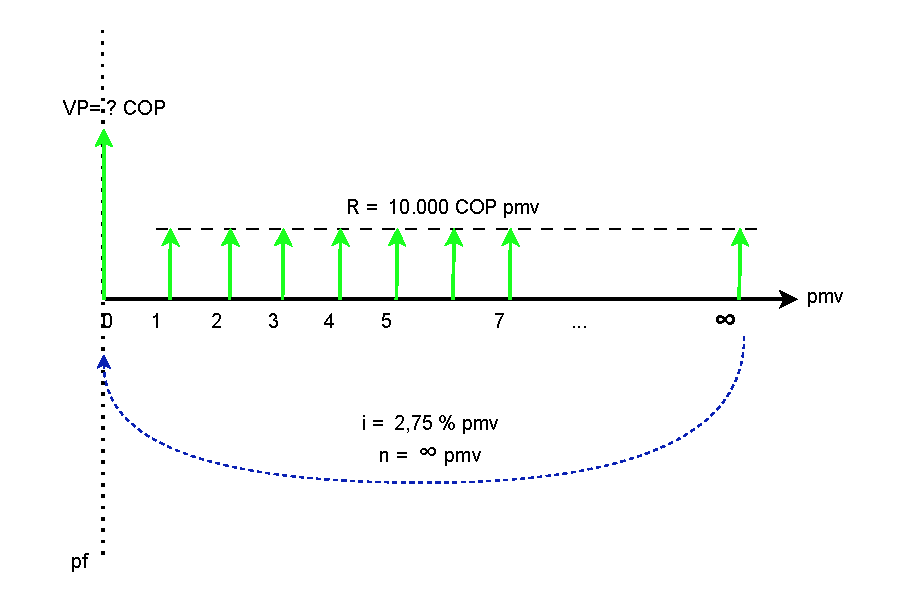
\includegraphics[trim=-5 -5 -5 -5 , width=9cm, height=8cm]{5_Capitulo/exportables/ejemplos/Capitulo5Ejemplo2.pdf}}   \\ \hline
		%%%%%%%%%%%%% FIN INSERCIÓN DE IMAGEN
		%%%%%FIN FLUJO DE CAJA
		
		
		
		%%%%% INICIO DECLARACIÓN FORMULAS
		%%%%%%%%%%% INICIO TITULO
		\rowcolor{orange!50}
		\multicolumn{3}{|c|}{\cellcolor{orange!50}\textbf{4. Declaración de fórmulas}}    \\ \hline
		%%%%%%%%%%% FIN TITULO
		%%%%%%%%%%% INICIO MATEMÁTICAS
		\multicolumn{3}{|c|}{$VP=\frac{R}{i}\hspace{0.3cm}\textit{Valor presente de una serie uniforme vencida perpetua}$} 	
		\\ \hline
		%%%%%%%%%% FIN MATEMÁTICAS
		%%%%%% INICIO DESARROLLO MATEMÁTICO
		\rowcolor{orange!50}
		%%%%%%%%%%INICIO TITULO
		\multicolumn{3}{|c|}{\cellcolor{orange!50}\textbf{5. Desarrollo matemático}}       \\ \hline
		%%%%%%%%%% FIN TITULO
		%%%%%%%%%% INICIO MATEMÁTICAS
		\multicolumn{3}{|c|}{$VP=\frac{10{.}000\,\,COP}{0.0275}=363{.}636,3636\,\,COP$}\\
		\hline
		
		
		%%%%%%%%%% FIN MATEMÁTICAS
		%%%%%% FIN DESARROLLO MATEMÁTICO
		%%%%%% INICIO RESPUESTA
		\rowcolor{orange!50}
		%%%%%%%%%%INICIO TITULO
		\multicolumn{3}{|c|}{\cellcolor{orange!50}\textbf{6. Respuesta}}   \\ \hline
		%%%%%%%%%% FIN TITULO
		%%%%%%%%%% INICIO RESPUESTA MATEMÁTICA
		\multicolumn{3}{|p{\textwidth}|}{\centering{El valor presente es de $363{.}636,3636\,\,COP$}}  \\ \hline
		%%%%%%%%%% FIN MATEMÁTICAS
		%%%%%% FIN RESPUESTA
	\end{longtable}
	%Se crean dos lineas en blanco para que no quede el siguiente texto tan pegado
	%\newline \newline %USARLO SI CREES QUE ES NECESARIO
\end{center}
%%%%%%%%%%%%%%%%%%%%%%%%%%FIN EJERCICIO 1 %%%%%%%%%%%%%%%%%%%%%%%%%%%
